\chapter{Procedimentos Metodológicos/Métodos e Técnicas}

Para o desenvolvimento deste trabalho serão realizadas as seguintes atividades:

\begin{itemize}

 \item Estudos dos algoritmos para a predição dos elementos regulatórios.

 Nesta etapa serão estudadas as técnicas de predição de elementos regulatórios.

 \item Implementação de métodos para a predição de elementos regulatórios.

Nesta fase, serão implementados os métodos mais significativos para a predição dos elementos regulatórios. Se algum algoritmo apresentar-se muito complexo exigindo um tempo de implementação que extrapolará o cronograma e havendo uma implementação do mesmo, de código livre, está será integrada na ferramenta, juntamente com os algoritmos implementados.


\item Integração dos algoritmos implementados, construindo uma ferramenta única para a predição dos elementos regulatórios.

Neste ponto, todos os algoritmos implementados serão agrupados em uma única ferramenta, para facilitar a utilização do usuário. A arquitetura da ferramenta proposta é descrita na figura \ref{fig:exec_alg}, onde podemos visualizar o esquema de funcionamento.

\begin{figure}[htb!]
    \centering
    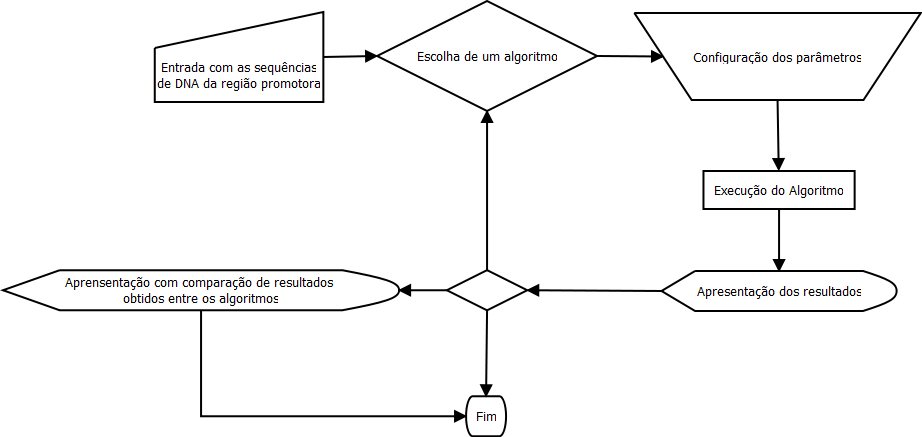
\includegraphics[scale=0.5]{./imagens/exec_alg.png}
    \caption{Esquema da funcionamento da ferramenta}
    \label{fig:exec_alg}
\end{figure}

 \item Validação dos elementos encontrados no genoma da soja.

Neste passo os elementos encontrados serão comparados com os elementos já existentes, avaliando a precisão dos métodos implementados.

\end{itemize}

Para implementação dos algoritmos será utilizada a linguagem de programação Python, devido ao grande desempenho desta linguagem e por oferecer um conjunto de métodos que facilita a manipulação de \textit{strings}.
